\documentclass[draft]{beamer}
\usepackage[T1]{fontenc}
\usepackage[utf8]{inputenc}
\usepackage[english]{babel}
\usepackage{graphicx,siunitx}
%Information to be included in the title page:
\title{Low jitter plasma channel in 3D printed gas filled capillary discharges}
\subtitle{Thesis Presentation}
\author{Ehud Behar}
\institute{Hebrew University of Jerusalem}
\date{2021}

\AtBeginSection[]
{
  \begin{frame}
    \frametitle{Table of Contents}
    \tableofcontents[currentsection]
  \end{frame}
} % put the table of contents at the beginning of each section and highlight the title of the current section

% from https://tex.stackexchange.com/a/415653/180429
\setbeamertemplate{frametitle continuation}{\insertcontinuationcount}
\begin{document}

\frame{\titlepage}
\begin{frame}
\frametitle{Table of Contents}
\tableofcontents
\end{frame}

\section{Theoretical Introduction}
\newcommand{\whatisplasma}{What plasma is?}
\begin{frame}{\whatisplasma}
Plasma is defined as an ionized gas of charged and neutral particles, which  satisfies  the quasi–-neutrality condition.
\begin{figure}
    \centering
    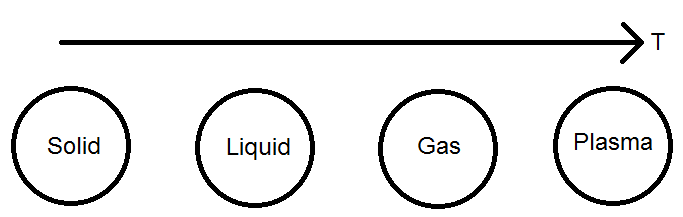
\includegraphics[width=0.5\textwidth]{presentation/temp_and_states.png}
\end{figure}
Molecules in the gas dissociate to form a gas of freely moving charged particles --- electrons and positive ions.
\end{frame}
\begin{frame}{\whatisplasma}
So, Plasma is a mixture of electrons, ions, and neutral particles moving in random directions that on the average is electrically neutral ($n_e \simeq n_i$).

In addition, plasmas are electrically conducting due to the presence of these free charge carriers and can attain electrical conductivities larger than metals such as gold and copper.
\end{frame}
\begin{frame}{Plasma characteristics}
It is customary to classify a plasma in terms of its electron temperature (measured in \si{\eV}) and electron densities (in \si{\per\cubic\cm}).
\vskip 1em
\begin{columns}
\column{0.5\textwidth}
One electron volt is equal to approximately \SI{11600}{\K}.
\column{0.5\textwidth}
Electron densities in the range \SIrange{e6}{e18}{\per\cubic\cm}
\end{columns}
\end{frame}
\section{The Spectrum of Hydrogen}
\newcommand{\hydrogenspecrum}{The Spectrum of Hydrogen}
\begin{frame}{\hydrogenspecrum}
    

An electron making a transition between two energy levels emits a photon.

Hydrogen spectrum is divided into series, determined by the transitions to the final state.
Balmer series:
\begin{itemize}
    \item $n_i=3 \to n_f=2$, \SI{656.3}{\nm} --- H\textsubscript{$\alpha$}
    \item $n_i=4 \to n_f=2$, \SI{656.3}{\nm} --- H\textsubscript{$\beta$}
\end{itemize}
Both H\textsubscript{$\alpha$} and H\textsubscript{$\beta$} are in the visible spectrum, and so are easy to observe.

Other series are Lyman ($n_f=1$) and Paschen ($n_f=3$).
\end{frame}
\begin{frame}{\hydrogenspecrum}
Spectroscopy study of such emission can give information about the physical conditions in the plasma, such as density and temperature.

Spectroscopic techniques have the advantage over some other methods -- those involving probes, for example -- that they do not interfere in any way with the plasma.

An inherent shortcoming of such observation is the fact that radiation is collected only along the line of sight in the direction of observation and any local information is therefore lost.
\end{frame}
\newcommand{\lte}{Local Thermodynamic Equilibrium(LTE)}
\begin{frame}{\lte}
    Electrons are energy providers for many plasma-chemical processes. The rate of such processes depends on the number of electrons having sufficient energy to do the job. This can be described by means of the electron energy distribution function f (e), which is a probability density for an electron to have the energy e. Quite often this distribution function strongly depends upon the electric field and gas composition, and can be very far from equilibrium. Sometimes, however, (even in nonequilibrium plasmas of nonthermal discharges), the f(e) depends mostly on electron temperature Te, and can then be defined by the quasi-equilibrium Maxwell–Boltzmann distribution function:
\end{frame}
\begin{frame}{Line Broadening}
A perfectly sharp energy line is impossible, and thus there is a distribution of transitions from states near $E_2$ to $E_1$.
    
\end{frame}
\end{document}